\documentclass[conference]{IEEEtran}
\usepackage{graphicx}
\usepackage{xspace}
\usepackage{syntax,etoolbox}
\usepackage{newfloat}
\usepackage{listings}
\usepackage{float}

%opening
\title{}
\author{}

\newcommand{\CodeIn}[1]{{\small\texttt{#1}}}
\newcommand{\dprle}{DPRLE\xspace}
\newcommand{\hampi}{HAMPI\xspace}
\newcommand{\zstr}{Z3-str\xspace}

\newcommand{\imss}{\CodeIn{IMSS}\xspace}


\begin{document}

\title{Integration of Multiple String Solvers}

\author{
    \IEEEauthorblockN{Siwakorn Srisakaokul, Wing Lam}
    \IEEEauthorblockA{Department of Computer Science, University of Illinois at Urbana-Champaign, Urbana, IL
        \\\{srisaka2, winglam2\}@illinois.edu}
}


\maketitle

\begin{abstract}
Many constraint solvers exist, each with their own strengths and weaknesses.
The burden to determine which solver is better equipped to handle regular expressions,
concatenations, context free grammar, and more has been on the users of these constraint
solvers. Not only are users expected to determine which solver may be compatible with
the constraints they would like to solve, users must learn how to express the
constraints they would like to solve in the language that corresponds to the constraint
solvers they would like to use.

A library has been developed to assist users from having to learn the language that
corresponds to the constraint solvers they would like to use.
This library proposes a common input and output for all constraint solvers.
However, this library requires the
developers of constraint solvers to integrate the library with their solvers.
The requirement of this cumbersome integration by developers results in
the limited adoption of this library. Not to mention the fact that even if a
constraint solver integrates such a library, it still continues to burden users to
determine which solver is best at solving particular constraints.

We designed and implemented \imss (Integration of Multiple String Solvers), a tool that
leverages the functionality of existing
constraint solvers to solve any constraint that existing solvers can solve in the
shortest amount of time. \imss accepts a set of constraints as input and translates the
input constraints into the language for other constraint solvers. Once the input
constraints are translated, \imss runs the constraint solvers it supports concurrently
to return satisfied or unsatisfied results to the user in the shortest amount of time.

\imss is lightweight and efficient, and can be easily enhanced to support
any constraint solver.
Our experiments use \imss with 3 renowned constraint solvers and compare each of
the constraint solvers' performance and results with other solvers.
\imss's source code, documentation, and the
experimental data are available at
https://github.com/winglam/Integration-of-Multiple-String-Solvers/.

%The language for \imss's input is expressive and efficient and can successfully
%represent any other constraint solver's language.

\end{abstract}

\section{introduction}
\label{sec:introduction}
HiHi

HiHi

\section{background}
\label{sec:background}

\newcommand{\dprletests}{16\xspace}
\newcommand{\hampitests}{379\xspace}
\newcommand{\ztests}{245\xspace}

This section describes the constraint solvers \imss supports and the concepts we used to develop \imss. The details of these solvers and and our tools are released on our project website~\cite{imss}.

\subsection{\hampi, \dprle, and \zstr}

\begin{figure}[H]
    \centering
    \begin{tabular}{|l|r|r|r|l|}
        %\toprule
        \hline
        \textbf{Constraint solver} & \textbf{LOC} & \textbf{Tests} & \textbf{Version} \\
        \hline
        \dprle & 2992 & \dprletests & 0.5.0\\
        \hampi & 14197 & \hampitests & 20120213\\
        \zstr & 8616 & \ztests & 1.0.0\\
        \hline
    \end{tabular}
    \caption{Constraint solvers supported by \imss.
        Column ``LOC'' represents the number of lines in the constraint solver's source code.
        Column ``Tests'' represents the number of tests provided by the developers of
        the constraint solvers.
    }
    \label{tab:solvers}
\end{figure}

\imss combines three different constraint solvers, \hampi, \dprle, and \zstr in order to
accept a wider range of languages as input and solve a greater variety of constraints.

\dprle is a decision procedure that solves constraints over regular languages. Regular languages
in \dprle are represented in the form of finite state automatas. \dprle constraints can express
membership and concatenation of regular languages~\cite{dprle2009}.
\imss currently supports the latest stable release of \dprle. This version of \dprle
includes \dprletests tests and all \dprletests tests were evaluated by \imss for our evaluation.

\hampi is a string constraint solver over fixed-size string variables. \hampi constraints can express
membership and may contain context-free language definition, strings, and regular-language
definitions~\cite{hampi2009}. Even though \hampi is a string solver over fixed-size string variables,
users can specify a range of lengths to \hampi, and \hampi will try all the lengths in the given range
and output the shortest string that satisfies the constraints.
\imss currently supports the latest stable release of \hampi. This version of \hampi
includes \hampitests tests and a subset of the \hampitests tests were evaluated by \imss for our evaluation.

\zstr, an extension of the Z3 SMT solver, is a string constraint solver that treats strings
as a primitive type and also supports booleans, integers, and string constants.
\zstr constraints can express variety of functionality such as concatenation, substring,
indexof, and replace~\cite{z32013}.
\imss currently supports the latest stable release of \zstr that was built with version
4.1.1 of Z3 (the most up to date version of Z3 \zstr is recommended to be built with).
This version of \zstr
includes \ztests tests and a subset of the \ztests tests were evaluated by \imss for our evaluation.

Given a set of constraints to \imss, \imss will translate the constraints to the format required by these three string solvers. These three string solvers will then output a string that satisfies the given constraints, or report that it is unsatisfiable.

\subsection{Abstract Syntax Tree}
Compilers typically consist of five main steps: lexical analysis, syntactic analysis, semantic
analysis, code generation, and optimization. Lexical analysis parses the source code which converting
a sequence of characters into a sequence of tokens. Then syntactic analysis will build a
Abstract Syntax Tree (AST) from the sequence of tokens. The AST is used to represent the structure
of the program. Each node of the tree denotes a statement or an expression in the source code.
The AST of the source code will be used in the next step, semantic analysis.
Semantic analysis, code generation, and optimization will do semantic checking, such as type checking,
then generate machine code instructions for the AST. Our tool, \imss, performs the first two steps.
The tool does not do type checking or code generation. Instead \imss takes a input constraint which can be
viewed as source code and translates it to a different format for the same source code.
It does this through lexical and syntactic analysis to generate an AST and then translating the AST (which captures all information of the source code) into three input formats
for the three solvers.

% Talk about AST
% Talk about the three solvers.
% Strengths and weaknesses of the solvers
% Statistics for number of tests for each solver

\section{approach}
\label{sec:approach}

\subsection{Overview Design of \imss}

\begin{figure}[H]
    \centering
    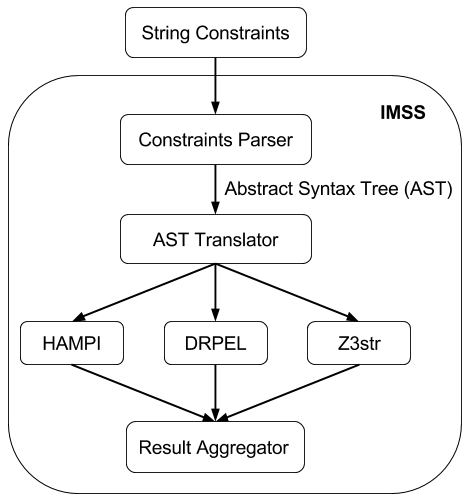
\includegraphics[scale=0.45]{imss}
    \caption{\label{fig:imss}Schematic view of \imss.}
\end{figure}

\imss finds a string that satisfies constraints specified in the input,
or decides that no satisfying string exists. \imss utilizes three different
string solvers: \hampi, \dprle, \zstr to solve string
constraints. In summary, \imss works in the following four steps (Figure~\ref{fig:imss}):
\begin{enumerate}
    \item Parse the input constraints into an abstract syntax tree (AST)
    representation of the \imss language.
    \item Translate the AST into the formats that corresponds to the three different solvers.
    \item Execute all the three solvers in parallel.
    \item Gather all the results. If none of the solvers can solve the constraints
    specified in the input, report that the constraints are incompatitble.
\end{enumerate}
The input format to \imss is specified by the grammar in Grammar~\ref{fig:grammar}.

\begin{Grammar}[H]
    \setlength{\grammarindent}{5em} % increase separation between LHS/RHS
    \begin{grammar}
        <Input> ::= <Statement>*                    \hfill \imss input

        <Statement> ::= String(<ID>)                \hfill string
                \alt Int(<ID>)                      \hfill int
                \alt StringDecl(<ID>, <STR_LIT>)    \hfill string witn value
                \alt Regex(<ID>, <RegStm>)          \hfill regex lang.
                \alt CFG(<ID>, <CFGStm>)            \hfill CFG lang.
                \alt <AssertStm>                    \hfill assert statement

        <RegStm> ::= <STR_LIT>                      \hfill string literal
                \alt <ID>                           \hfill variable name
                \alt Fix(<ID>, <INT_LIT>)           \hfill CFG fixed-sizing
                \alt Or(<RegStm>*)                  \hfill union
                \alt Concat(<RegStm>*)              \hfill concatenation
                \alt Star(<RegStm>)                 \hfill Kleene star

        <AssertStm> ::= AssertIn(<ID>,<ID>)         \hfill membership
                \alt Equal(<Exp>,<Exp>)             \hfill string equality
                \alt Contains(<StrExp>,<StrExp>)    \hfill string contains

        <Exp> ::= <IntExp>                          \hfill integer expression
                \alt <StrExp>                       \hfill string expression
                \alt <RegExp>                       \hfill regex expression
                \alt <ID>                           \hfill variable name

    \end{grammar}
 \caption{\label{fig:grammar}Subset of \imss's input language, shown in BNF grammars.
 Non-terminals are shown in angle brackets. \imss's input consists of a list of statements.
 Statements can be variable declaration or assertion statements which represent
 string constraints.}
 \end{Grammar}

\subsection{Example}

In order to demonstrate the four steps of \imss, consider the example below:
\renewcommand\lstlistingname{Code}
\begin{lstlisting}[label={code:example},frame=bt,numbers=none,basicstyle=\ttfamily\scriptsize,
language=C,captionpos=b,caption={Input constraint in \imss format}]
1.  String(v);
2.  RangedLength(v, 1, 100);
3.  Contains(v, "abc");
5.  Regex(r, Star(Or("ab", "cd")))
6.  Contains(v, "deg");
7.  AssertIn(v, r);
6.  SolveAll();
\end{lstlisting}
This is a constraint for a string that contains the substring $abc$, and
the string is a member of the regular expression, $(ab|cd)*$.
One of the strings which satisfy this constraint is ``abcd''. The string can be of any length
between 1 and 100. \imss will parse the input into an AST (Figure~\ref{fig:exp-ast}) according to Grammar~\ref{fig:grammar}.

\begin{figure*}
    \centering
    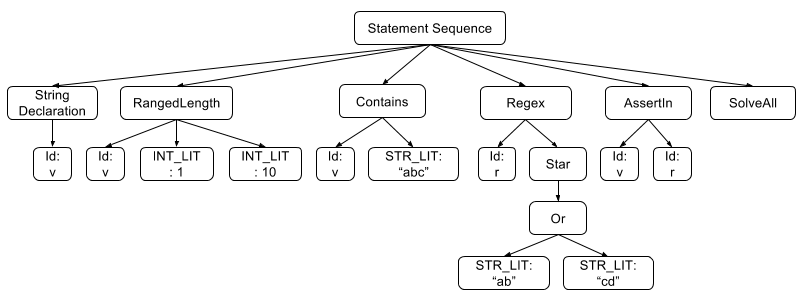
\includegraphics[scale=0.65]{example-ast}
    \caption{\label{fig:exp-ast}Abstract syntax tree of the example Code~\ref{code:example}.}
\end{figure*}

Then, \imss will translate the AST into all three input formats by traversing the tree and
translating each tree node into the string format for each language. If a language does not support
some functionality (\imss cannot translate some node into that specific language),
then translation to that language will fail and \imss will output ``incompatible'' for that language. After the translations, \imss executes all of the generated input formats
on its corresponding solver in parallel and outputs the fastest solution (or all solutions depending on the configuration for \imss).

% Internal representation that we generate with our inputs and how we convert the
% representation to the three outputs. Provide an cool example if possible.
% Provide the list of commands we support if necessary/helpful.
% Translation for how we got our input (?)

\section{implementation}
\label{sec:implementation}
In this section we will explain in-depth the implementation of \imss.
The architecture of \imss is shown
in Figure~\ref{fig:imss}. The tool takes string constraints in \imss format
and generates at least one output that satisfies the given constraints if the constraints are satisfiable.
\imss is implemented in Java and uses three different solvers to satisfy its input constraints.


\subsection{\imss's Grammar}
Since, \hampi, \dprle, and \zstr takes their inputs in
 different languages. These three languages do not have the same expressiveness.
 We cannot use translate everything from one language into the other two languages. For example,
 \dprle, requires automata descriptions for its input~\cite{lazystrings2010}.
 To define a string, we have to construct a finite automaton representing that string.
 Also, \dprle, does not support a constraint which has a context-free grammar,
 but \hampi does. However, \dprle, can check whether one regular expression language
 contains another regular expression language. Each language has some functionalities the
 other solvers do not have. Thus, we construct a new grammar (Grammar~\ref{fig:grammar}) that is expressive enough to
 cover all the functionalities in all three languages by combining their grammars.

\subsection{Input Format Translation}
After \imss takes a input constraint in \imss's format, it constructs an AST representation of the input.
Each AST node stores its type, according to the grammar, and pointers to its child nodes.
For example, the AST of \CodeIn{LessThan(a, 2)} consists of three nodes. The root node is of type
\CodeIn{LessThan} and that node has two children. In this example, the first child is of type \CodeIn{ID} (variable name), and
the second child is of type \CodeIn{INT_LIT}. We infer the types from \imss's grammar.
With this approach, every tree node has an associated type. Given the type information of
each AST node, we can easily translate this tree into the three different languages by traversing
on the tree and recursively constructing the input constraints for each of the three languages.

\subsection{Result Aggregation}
After \imss generates the input constraints for each language, it executes the three solvers concurrently, and
reports a string that satisfies the given constraint, assuming at least one solver can handle the input.


\section{evaluation}
\label{sec:evaluation}

\begin{figure}[H]
    \centering
    \begin{tabular}{|l|c|c|c|}
        \hline
        \textbf{Constraint solver} & \dprle & \hampi & \zstr \\
        \hline
        \multicolumn{4}{|l|}{}  \\
        \multicolumn{4}{|l|}{\textbf{\dprle tests}}  \\
        \hline
        SAT & 14 & 2 & 2 \\
        UNSAT & 0 & 0 & 0 \\
        Incompatible & 2 & 14 & 14 \\
        \hline
        \multicolumn{4}{|l|}{}  \\
        \multicolumn{4}{|l|}{\textbf{\hampi tests}}  \\
        \hline
        SAT & 3 & 49 & 12 \\
        UNSAT & 0 & 20 & 2 \\
        Incompatible & 66 & 0 & 55 \\
        \hline
        \multicolumn{4}{|l|}{}  \\
        \multicolumn{4}{|l|}{\textbf{\zstr tests}}  \\
        \hline
        SAT & 5 & 3 & 38 \\
        UNSAT & 0 & 1 & 8 \\
        Incompatible & 41 & 42 & 0 \\
        \hline
    \end{tabular}
    \caption{
        For each solver's set of tests, this table shows the number of tests each solver
        is incompatible with and for compatible tests, what the output of those tests
        are.
    }
    \label{tab:solvercompareresults}
\end{figure}

\begin{figure}[H]
    \centering
    \begin{tabular}{|l|c|c|c|}
        \hline
        \textbf{Constraint solver} & \dprle & \hampi & \zstr \\
        \hline
        \dprle & 1.00 & 30.52 & 13.03 \\
        \hampi & 0.04 & 1.00 & 0.40 \\
        \zstr & 0.31 & 11.91 & 1.00 \\
        \hline
    \end{tabular}
    \caption{
        This table shows the increase or decrease in time for the solvers to solve the
        same constraints.
        The data in each cell is calculated by taking the average time the solver
        represented by the row took to solve the tests belonging to the solver represented
        by the column over the average time the solver represented by the column
        took to solve the same tests. A number less than 1 represents a decrease in time.
    }
    \label{tab:solvercomparetime}
\end{figure}

% Translation for how we got our input (?)
% Show the two charts.
% Show how some of DPRLE's tests do not work for DPRLE
% Timing for how some of Z3's tests takes almost 4 times longer
% to run on Hampi.
% All solvers reported correct output

\section{related works}
\label{sec:related}

Boolector is an efficient SMT solver for the quantifier-free theory
of bit-vectors in combination with the extensional theory of arrays~\cite{boolector2009}.
Boolector depends on term rewriting and bit-blasting for bit-vectors. It
takes a formula expressed in the SMT-LIB format~\cite{smtlib2015}, or alternatively in
the BTOR format~\cite{btor2008}, as input.
The BTOR format is a low-level bit-vector format with clean semantics that is easy to
parse. Additionally, BTOR supports bit-vector arrays and model checking of safety
properties.
Aside from being an SMT solver, Boolector contains a tool known as
Pretty Printer. Pretty Printer allows Boolector to convert formulas from BTOR to
SMT-LIB format and vice versa. The Pretty Printer can be combined with Boolector’s
rewriting module to internally simplify the formula before conversion.
Pretty Printer is the only existing tool (to the best of our knowledge) that is capable of
converting from one language format to another for constraint solving purposes.
While Pretty Printer can convert between 2 languages, \imss is able to convert
between 4 different languages with many more planned to be added soon.

SMT-LIB is an international initiative aimed at facilitating research and development in
Satisfiability Modulo Theories (SMT)~\cite{smtlib2015}. Since its inception in 2003, the
initiative has focused on 5 concrete goals. One of these goals is to develop and promote
common input and output languages for SMT solvers.
SMT-LIB has accomplished this by providing a way for developers of constraint solvers
to integrate SMT-LIB with their solvers.
Compared to \imss, \imss does not require developers of constraint solver to
do anything and it alleviates the burden users have in
determining which solver is best at solving particular constraints.

% Need to talk about SMT-lib, search on Google scholar for other similar projects to ours

\section{conclusion}
\label{sec:conclusion}
We presented \imss, a solver for string constraints. \imss is the integration of
multiple solvers: \hampi, \dprle, and \zstr. \imss constraints can express
membership and string function such as replace, length, contains, and substring. The constraints
can contain arbitrary string variables, context-free language definitions, integers,
and regular language definitions. Given string constraints, \imss outputs
a string that satisfies the constraints, or reports that the constraints are incompatible.
By using \imss, users do not have to decide which solver from the three solvers
they should use to solve their constraints.

We evaluated \imss on the 131 derived tests we picked such that they contain all the functionalities
that the three solvers have together. Our experiment shows that \imss can solve all the tests
within a reasonable running time.

\dprle is the fastest solver, but it lacks of many functionalities. \zstr can solve
the most number of string constraints without context-free grammar definitions which only
\hampi supports.
\ping{Wing, talk about future works}

% Should talk about future work somewhere
% !) Complete translation of all of the solver's tests
% 2) Automatic translation the other solver's language to our language
% 3) Accepting SMT-Lib's format as input to support ALL solvers that support SMT-Lib
% 4) Adding other solvers such as Kaluza
% 5) Constraint Analyzer that uses heuristics to determine which solvers to only run
% 6) Use a constraint generator and test which solver is best at solving such constraints

\bibliographystyle{IEEEtran}
\bibliography{references}

\end{document}
